%    Copyright (C)  2011  Santiago Gutierrez Alzate, Sebastian Gomez Gonzalez.

%    Permission is granted to copy, distribute and/or modify this document
%    under the terms of the GNU Free Documentation License, Version 1.3
%    or any later version published by the Free Software Foundation.
%    A copy of the license is included in the section entitled "GNU
%    Free Documentation License" in spanish.

%    Se concede permiso para copiar, distribuir y/o modificar este documento bajo 
%    los términos de la Licencia de Documentación Libre de GNU, Versión 1.3 o 
%    cualquier otra versión posterior publicada por la Free Software Foundation;
%    Una copia de la licencia está incluida en la sección titulada GNU Free
%    Documentation License.


\documentclass[a4paper, 11pt, oneside]{report}

% idioma
\usepackage[utf8]{inputenc}
\usepackage[spanish]{babel}

%tablas
\usepackage{booktabs}

%rotar tablas
\usepackage{rotating}

%color tablas
\usepackage{colortbl}



%espaciado
\usepackage{setspace}
\onehalfspacing
\setlength{\parindent}{0pt}
\setlength{\parskip}{2.0ex plus0.5ex minus0.2ex}


%margenes según n. icontec
\usepackage{vmargin}
\setmarginsrb           { 4.0cm}  % left margin
                        { 3.0cm}  % top margcm
                        { 2.0cm}  % right margcm
                        { 2.0cm}  % bottom margcm
                        {   0pt}  % head height
                        {0.0 cm}  % head sep
                        {   9pt}  % foot height
                        { 1.0cm}  % foot sep

% inserción url's notas de pie.
\usepackage{url}

%gráficos
\usepackage{graphicx}

% Paquetes de la AMS:
\usepackage{amsmath, amsthm, amsfonts}
\addto\captionsspanish{\def\refname{\textsc{Bibliografía}}}

\newcommand\portada{
	\begin{titlepage}
		\begin{center}
			{\large \bf DESARROLLO DE UN SISTEMA PROTOTIPO DE RECONOCIMIENTO DE DÍGITOS USANDO MOMENTOS INVARIANTES }
			\vfill
% 			{\large\bf PRESENTADO POR \par}
			{\large\bf SEBASTIÁN GÓMEZ GONZÁLEZ \par}
			{\large\bf SANTIAGO GUTIERREZ ALZATE \par}
			\vfill
			{\large\bf UNIVERSIDAD TECNOLÓGICA DE PEREIRA  \par}
			{\large\bf FACULTAD DE INGENIERÍAS \par}
			{\large\bf INGENIERÍA DE SISTEMAS Y COMPUTACIÓN \par}
			{\large\bf PEREIRA\par}
			{\large\bf SEPTIEMBRE DE 2010 \par}
		\end{center}
	\end{titlepage}
}

\newcommand\contraportada{
	\begin{titlepage}
		\begin{center}
			{\large \bf DESARROLLO DE UN SISTEMA PROTOTIPO DE RECONOCIMIENTO DE DÍGITOS USANDO MOMENTOS INVARIANTES }
			\vfill
% 			{\large\bf PRESENTADO POR \par}
			{\large\bf SEBASTIÁN GÓMEZ GONZÁLEZ \par}
			{\large\bf SANTIAGO GUTIERREZ ALZATE \par}
			\vfill
			{\large\bf INFORME DE PROYECTO DE GRADO DE PREGRADO\par}
			\vfill
			{\large\bf UNIVERSIDAD TECNOLÓGICA DE PEREIRA  \par}
			{\large\bf FACULTAD DE INGENIERÍAS \par}
			{\large\bf INGENIERÍA DE SISTEMAS Y COMPUTACIÓN \par}
			{\large\bf PEREIRA\par}
			{\large\bf SEPTIEMBRE DE 2010 \par}
		\end{center}
	\end{titlepage}
}

\graphicspath{./diagrams/}

\begin{document}
\portada
\contraportada

\tableofcontents


\chapter{Introducción}
\label{chap:intro}

\section{Descripción del problema}

Los problemas visuales afectan a una gran parte de la población, tanto en Colombia\footnote{Según el DANE en su gran censo nacional realizado en el año 2005, se estima que el 6.3\% de la población colombiana sufre de alguna discapacidad. De estas personas con discapacidad se estima que el 43.4\% tienen dificultades para ver aun con lentes.} como a nivel mundial\footnote{La organización mundial de la salud estima que en el mundo hay 161 millones de personas con problemas visuales, de los cuales 37 millones son ciegos.}, estos traen consigo consecuencias devastadoras para las personas que los sufren, afectando su calidad de vida significativamente. Entre todos los problemas que sufren las personas con discapacidades visuales, uno de los más críticos es el del acceso a la información; esto debido a que la mayoría de la información los seres humanos reciben del entorno llega a través de los ojos. Los problemas para obtener información causan que las personas con discapacidades visuales se queden rezagadas con respecto a los demás miembros de la sociedad, impidiendo así que tengan las mismas oportunidades de vida que una persona con sus cinco sentidos intactos. Generalmente, esto causa un efecto de exclusión y de segregación en estas personas debido a que son vistas como una carga, tanto por si mismas como por las personas que los rodean. 

A partir de la incidencia del problema, una forma de ayudar a que las personas con discapacidades visuales tengan una mejor calidad de vida es lograr que puedan tener acceso a la información que se encuentra en documentos escritos, tales como cartas, libros, y volantes. Esto puede ser logrado a través un sistema de reconocimiento óptico de caracteres que reconozca el texto escrito en estos documentos y le lea a la persona invidente lo que dicen. Sin embargo, para que sea una solución efectiva al problema, se requiere de un sistema que le permita a los discapacitados visuales acceder a la información escrita de una manera rápida y fácil, lo cual implica gran movilidad. Si bien existen múltiples sistemas de reconocimiento óptico de caracteres para computadores de escritorio, estos no poseen dicha movilidad, porque además del computador, también necesitan de un escáner para funcionar. Así pues, para que un sistema de este tipo pueda ser utilizado en múltiples lugares, se requiere de algún dispositivo que sea: pequeño, fácilmente transportable y capaz de hacer el trabajo en un tiempo razonable. Los teléfonos inteligentes parecen ser una buena alternativa, no obstante, existen grandes diferencias entre un computador de escritorio y un teléfono inteligente, entre ellas se pueden resaltar las siguientes:

\begin{itemize}

\item La memoria y la capacidad de procesamiento son muy reducidas en los teléfonos inteligentes con respecto a los computadores de escritorio.

\item El tamaño de la memoria cache es mucho más pequeño en los teléfonos inteligentes. Como resultado de esto, los algoritmos diseñados para computadores de escritorio pueden ser muy lentos en los teléfonos inteligentes, pues se hicieron pensando en caches de varios megabytes.

\item Un computador de escritorio normalmente tiene instaladas múltiples librerías de propósito general que son utilizadas por distintos programas, un teléfono inteligente, en cambio, solo provee las librerías más básicas.

\end{itemize}

La diferencia más importante, sin embargo, es que en los computadores de escritorio las imágenes son obtenidas por medio de un escáner, logrando condiciones de iluminación muy buenas y uniformes, mientras en los teléfonos inteligentes las imágenes se obtienen por medio de una cámara fotográfica. Esta diferencia es muy importante para el reconocimiento óptico de caracteres, en especial si quien toma la foto es una persona invidente, ya que en este caso diversas variables como la inclinación del texto, la iluminación no uniforme, y las deformaciones elásticas del texto debido a la forma del papel en reposo, cobran más relevancia, pues la persona invidente podría tomar la fotografía inclinada, en el sentido contrario, o en un lugar con poca luminosidad.

Para dar solución al problema de limitación en la capacidad de procesamiento de los teléfonos inteligentes se puede utilizar una de sus grandes ventajas: son por naturaleza dispositivos de alta conectividad. Cada vez los planes de telefonía son más económicos y hay más disponibilidad de redes inalámbricas, a las cuales los teléfonos inteligentes tienen acceso, en diferentes sitios públicos como institutos educativos y bibliotecas. Esta alta conectividad posibilita la construcción de un sistema de reconocimiento óptico de caracteres con una arquitectura cliente-servidor, en la cual el teléfono inteligente pueda enviar la imagen por internet y esta sea procesada por un servidor con una capacidad de cómputo mucho mayor. Este sistema tendrá las mismas ventajas de movilidad y rapidez deseadas. La capacidad de procesamiento de los celulares inteligentes también ha incrementado en los últimos años, lo que permitiría hacer parte del procesamiento en el celular, con el objetivo de reducir el ancho de banda requerido para enviar la imagen al servidor y por tanto el costo.

Para solucionar los problemas asociados con la inclinación del texto que se puede producir en las imágenes tomadas por la persona invidente, se hace necesario un sistema de reconocimiento óptico de caracteres que pueda reconocer exitosamente fotos tomadas con distintos grados de inclinación o incluso en el sentido contrario.

Después de una búsqueda en más de 20 artículos científicos relacionados al tema de reconocimiento óptico de caracteres, y de revisar la documentación técnica de varios OCRs libres, no se encontró un sistema de reconocimiento de caracteres por un medio óptico que haya sido desarrollado para ser usado por personas invidentes en teléfonos inteligentes, que sea de código libre y abierto, y que solucione los problemas de inclinación y luminosidad antes presentados. 

\subsection{Definición del problema}

No existe \footnote{ZHOU, Steven; SYED, Gilani y WINKLER, Stefan. Open Source OCR Framework Using Mobile Devices. MULTIMEDIA ON MOBILE DEVICES (1: 28-29 enero, 2008: San José, California, Estados Unidos). Memorias, 2008, vol. 6821, p. 41-46} un sistema de reconocimiento óptico de caracteres que halla sido desarrollado para ser utilizado por personas invidentes utilizando la cámara de celulares inteligentes, que sea de código abierto, y con un porcentaje de reconocimiento satisfactorio.

\section{Justificación del proyecto}

Un sistema móvil para reconocer texto de documentos impresos presentaría los siguientes beneficios respecto de los sistemas tradicionales como las impresoras braille y los lectores basados en escáner:

	\begin{itemize} 

	\item Un menor costo, al no ser necesario adquirir un computador de escritorio, escáner o impresora braille.

	\item Portabilidad: ninguno de los sistemas tradicionales esta diseñado para ser llevado en todo momento por el usuario, dificultando el acceso al conocimiento e información que no se encuentre en el lugar físico en el que se encuentra alguno de estos sistemas.
	
	\item Una solución económica que pueda ejecutarse en un dispositivo móvil, sin necesidad de hardware adicional, haría posible que cada invidente pudiera tener su propio sistema de OCR personal, mientras que los otros sistemas usualmente (por su costo) son adquiridos por instituciones en cantidad limitada.

	\item Aportar al conocimiento: Al desarrollar este aplicativo se tendrán que hacer pruebas experimentales cuyos resultados aporten a otras investigaciones.

	\end{itemize}
	
\section{Objetivo}
\label{sect:objective}
	
	\subsection{Objetivo general}
	Desarrollar un sistema prototipo de reconocimiento óptico de dígitos numéricos bajo condiciones especificadas, usando para el reconocimiento una distribución normal multivariable con el teorema de Bayes y un vector de características invariantes (momentos de Hu y Fluzzer).
	\subsection{Objetivos específicos}
	\begin{itemize}
	\item Realizar un estudio del funcionamiento de la distribución normal multivariable en el problema de reconocimiento usando el teorema de Bayes.
	\item Realizar la extracción de características de un conjunto de imágenes de dígitos. Las características a extraer serán invariantes a la rotación, translación y escalamiento (Momentos de Hu y Fluzzer).
	\item Diseñar e implementar una aplicación que integre estos algoritmos y permita el reconocimiento óptico de dígitos.
	\item Realizar pruebas de la aplicación implementada.
	\item Realizar un análisis comparativo de los resultados obtenidos.
	\end{itemize}
	
\section {Antecedentes}

La tecnología actual ha permitido a las personas invidentes tener acceso a información y a conocimiento al que antes no tenían acceso. Entre estas tecnologías se encuentran los lectores de pantalla, y las impresoras y sistemas refrescables de Braille.
	
Un proyecto interesante desarrollado en la Universidad Tecnológica de Pereira (llamado Proyecto IRIS), permite a los invidentes reconocer imágenes con colores a través de vibraciones a diferentes frecuencias. Para lograrlo se utiliza un guante con imanes permanentes y una matriz de electroimanes conectada al computador por el puerto USB.

En el área de acceso al texto, existen sistemas que convierten el texto en ASCII a voz, conocidos como sistemas \textit{Text-To-Speech}. También existen sistemas para el computador que permiten pasar texto en imagen a texto en ASCII, conocidos como OCR, los cuales funcionan usualmente tomando una imagen de un escáner. Según pruebas de eficacia realizadas por la TUK \footnote{BREUEL, Thomas. The OCRopus Open Source OCR System. DOCUMENT RECOGNITION AND RETRIVAL. (15: 29-31, febrero, 2008: San José, Estados Unidos). Memorias, 2008, p. 68-150}, los OCRs libres con mejores resultados son \textit{Tesseract} y el  \textit{Ocropus}. 

Cuando el problema cambia de tomar la imagen con un escáner a tomarla con una cámara, se deben seguir diferentes enfoques, en \footnote{SMITH, Ray. Progress in Camera-Based Document Image Analysis. INTERNATIONAL CONFERENCE ON DOCUMENT ANALYSIS AND RECOGNITION (7: 3-6, agosto, 2003: Edimburgo, Escocia). Memorias, 2003, p. 606-617} se halló que los retos más importantes son la proyección de la imagen en perspectiva en el plano y la  resolución requerida para poder reconocer bien los caracteres.

En cuanto a hacer que el OCR sea realizado por un celular, se encontraron investigaciones como \footnote{ZHOU, Steven; SYED, Gilani y WINKLER, Stefan. Open Source OCR Framework Using Mobile Devices. MULTIMEDIA ON MOBILE DEVICES (1: 28-29 enero, 2008: San José, California, Estados Unidos). Memorias, 2008, vol. 6821, p. 41-46}, en la que se trabajaban con imágenes de muy baja resolución (640x480) y como resultado solo pueden reconocer textos muy cortos, tales como avisos y carteles, pero no documentos completos. En \footnote{SENDA, Shuji, et al. Camera-Typing Interface for Ubiquitous Information Services. IEEE ANNUAL CONFERENCE ON PERVASIVE COMPUTING AND COMMUNICATIONS (2: 14-17, marzo, 2004: Orlando, Florida, Estados Unidos). Memorias, 2004, p. 366-372}, para tratar de equilibrar el hecho de tener una cámara de baja resolución, se toman varias imágenes de baja resolución en lugar de una sola, uniéndolas posteriormente para lograr una mejor resolución. Esto sin embargo conlleva a un incremento la carga de procesamiento, haciendo que no sea posible el procesamiento dentro del celular, por lo cual la solución se restringe para que se envíen las imágenes a un servidor usando internet, el cual las procesa y envía los resultados.

Cabe anotar que ninguna de las tecnologías anteriormente mencionadas para hacer el OCR en el celular fue diseñada para ser usada por personas invidentes. Ya que el primero no fue diseñado para reconocer documentos, y el segundo requeriría que la persona invidente supiera con anterioridad como está la estructura del documento para poder mover la cámara del celular en la dirección en la que está el texto en el documento.
	
\subsection{Proyectos de grado relacionados en la Universidad Tecnológica de Pereira}

Si bien en Ingeniería de Sistemas en la Universidad Tecnológica de Pereira no se ha planteado un proyecto de grado directamente sobre reconocimiento óptico de caracteres, un estudiante de la maestría en Ingeniería Eléctrica construyo un sistema para el reconocimiento de algunos caracteres y dígitos manuscritos. Se intentaron dos maquinas de aprendizaje diferentes: el perceptrón multicapa (comúnmente conocido como red neuronal) y la maquina de vectores de soporte. Sus resultados demostraron que las maquinas de vectores fueron superiores a las redes neuronales en todas las pruebas, así que estas maquinas de aprendizaje podrían ser de gran utilidad en la construcción de un sistema de reconocimiento óptico de caracteres. \footnote{MUÑOZ, Pablo Andrés. Máquinas de aprendizaje para reconocimiento de caracteres manuscritos. Tesis de Maestría en Ingeniería Eléctrica. Pereira: Universidad Tecnológica de Pereira, 2005}

En temáticas relacionadas, se encontraron los siguientes proyectos de grado desarrollados por estudiantes de Ingeniería Eléctrica:
    
En la tesis \footnote{RINCÓN, Jaime; LOAIZA, Johan Eric. Reconocimiento de palabras aisladas mediante redes neuronales sobre FPGA. Trabajo de grado Ingeniero Electricista. Pereira: Universidad Tecnologica de Pereira, 2008} se utilizaron redes neuronales para reconocimiento de voz en hardware sobre una FPGA. Si bien la implementación fue en hardware y no en software, sus resultados permiten inferir que es posible implementar maquinas de aprendizaje sofisticadas (como las redes neuronales) con un bajo uso de memoria y con relativa eficiencia, lo cual da esperanzas para una posible implementación de las misma en un dispositivo móvil. También es de anotar que las redes neuronales demostraron porcentajes de aciertos significativamente mayores que los obtenidos por los clasificadores bayesianos lineales.

En el tema de procesamiento de imágenes, se encontró un proyecto de grado para contar transeúntes en una imagen utilizando un sistema de visión artificial \footnote{VALENCIA, Joan Mauricio; ABRIL Mauricio. Registro de transeúntes en tiempo real utilizando un sistema de visión artificial sobre un ambiente controlado. Trabajo de grado Ingeniero Electricista. Pereira: Universidad Tecnologica de Pereira, 2007}. Considerando el bajo nivel de resolución (imágenes de 324 x 240 píxeles a 30 frames por segundo) y el hecho de que la cámara no fue calibrada, se identificaron correctamente muchos transeúntes, de lo que se puede inferir que los sistemas de visión artificial funcionan correctamente con cámaras económicas. Los resultados muestran que el uso de histogramas puede ser de gran utilidad a la hora de distinguir componentes conectados de píxeles. Así mismo, también permiten entender distintos problemas que se pueden presentar a la hora de separar estos componentes correctamente, como por ejemplo la identificación de varios transeúntes como uno solo. Si bien en el reconocimiento óptico de caracteres se distinguen letras y no personas, problemas similares a los evidenciados en este proyecto se presentan al separar los caracteres en un sistema de OCR.
	
Finalmente, en el tema de procesamiento de señales, en \footnote{ALVAREZ, Lorena. Acondicionamiento de Señales Bioeléctricas. Trabajo de grado Ingeniero Electricista. Pereira: Universidad Tecnologica de Pereira, 2007} se adquieren señales bioeléctricas utilizando filtros análogos y digitales. En este proyecto se lograron filtrar señales muy pequeñas y finas, como las producidas en el cuerpo humano, mediante filtros digitales, y se obtuvieron errores pequeños. Aunque las señales bioeléctricas son muy diferentes a las imágenes, es posible convertir estas ultimas en señales y, por tanto, los filtros digitales expuestos en este proyecto podrían ser de utilidad a la hora de eliminar errores en imágenes tomadas por una cámara, ya que logran filtrar correctamente señales con gran cantidad de ruido.\newline
    
\section {Modelo general de sistema OCR}

\subsection{Reconocimiento de caracteres y análisis de documentos}

En esta sección se hablará de algunas investigaciones realizadas en el área de reconocimiento de caracteres y de análisis de documentos. Las etapas necesarias para llevar a cabo el proceso de análisis de documentos y reconocimiento de caracteres son: binarización de la imagen, análisis y segmentación del documento y reconocimiento óptico de caracteres (OCR).  

\subsection{Binarización de imagen}

Esto se refiere a tomar una imagen en escala de grises y convertirla a una  imagen en blanco y negro. También se puede ver como separar la parte que nos interesa (foreground o primer plano) de la parte que no nos interesa (background o fondo). Una técnica que da buen resultado es la binarización de Sauvola, que realiza una binarización basada en un análisis local de la imagen. El hecho de que sea local le brinda una mejor binarización en condiciones de luz variable. Los  resultados obtenidos en el artículo "Efficient Implementation of Local Adaptative  Thersholding Techniques Using Integral Images" indican que esta técnica puede ser optimizada para lograr un tiempo de ejecución comparable con las técnicas globales de  binarización (al correr en O(N) \footnote{La función $O(f)$ se usa para indicar que la complejidad algorítmica es una función $f(N)$ que depende de la talla del problema $N$. Sea $T(N)$ el tiempo de  ejecución del algoritmo para una talla de problema $N$, entonces existe una constante $K$ tal que  $\forall N ( K*f(N) < T(N) ) $}, siendo N el numero de píxeles de la imagen), conservando	las ventajas de ser local, por lo que seria un buen candidato para implementarlo en un  proyecto para desarrollar un sistema de reconocimiento óptico de caracteres.

\subsection{Análisis del documento}

Según \footnote{MAO Song; AZRIEL, Rosenfelda y KANUNGOB, Tapas. Document structure analysis algorithms: A literature survey. DOCUMENT RECOGNITION AND RETRIVAL. (10: enero, 2003: San José, Estados Unidos).  Memorias, 2003, p. 197-207}, esta etapa puede ser vista como un análisis sintáctico, en el que el documento se divide en sus partes estructurales como un árbol de análisis sintáctico. Como todo análisis gramatical, se puede seguir los enfoques \textit{buttom-up} y \textit{top-down}. Un enfoque \textit{buttom-up} comenzaría desde los píxeles y luego los relacionaría en grupos mas grandes (Caracteres, Palabras, Lineas o Párrafos). Un enfoque \textit{top-down} por el contrario, comienza con la imagen de un documento y comenzaría a dividirla hasta llegar a sus componentes. Cada algoritmo tiene limitaciones, ventajas y distintos requerimientos de máquina. Una investigación realizada sobre diferentes algoritmos \footnote{SHAFAITA Faisal; KEYSERSA,  Daniel y BREUEL, Thomas. Performance Evaluation and Benchmarking of Six-Page segmentation Algorithms. \underline{En}: IEEE Transactions on Pattern Analysis And Machine Intelligence.  Junio, 2008. vol. 30, no. 6, p. 941-954}, indica que los mejores resultados sobre diferentes documentos, con distintas estructuras físicas, fueron para Docstrum y para Voronoi, con porcentajes de error del 4.3\% y 4.7\% respectivamente. Otro método	llamativo es el \textit{RLSA}, que llama  la atención por su sencillez y puede brindar buenos resultados en documentos \textit{Manhattan-Layout}. 

Probablemente la mejor solución para un sistema OCR pueda resultar de la mezcla de varios de los algoritmos existentes, en \footnote{KISE, Koichi; SATO Akinori y MATSUMOTO,  Keinosuke. Document Image Segmentation as Selection of Voronoi Edges. IEEE COMPUTER SOCIETY: CONFERENCE ON COMPUTER VISION AND PATTERN RECOGNITION (66: 17-19, junio, 1997: San Juan,  Puerto Rico). Memorias, 1997, p. 32-39} se observa como se pueden mejorar los resultados  mezclando los beneficios de diferentes algoritmos para soluciones particulares, y cada uno de los artículos mencionados aporta elementos importantes para escoger cual de estos algoritmos  es ventajoso para una solución particular.  

\subsection{Reconocimiento óptico de caracteres OCR}

Esta etapa se puede clasificar como un subproblema del reconocimiento de patrones. Existen varias aproximaciones para solucionar el problema de reconocimiento de patrones. Entre ellos algunos modelos son inspirados en la biología, como los que usan redes neuronales. Otros modelos son puramente matemáticos como las máquinas de vectores de soporte, o estadísticos como la distribución normal multivariable aplicando el teorema de Bayes.

La  mayoria de los métodos para el reconocimiento de patrones tienen en común que necesitan como entrada un vector de características. Para el problema de reconocimiento de dígitos o caracteres para las personas invidentes, es deseable que estas características cambien muy poco frente a ciertos cambios en la imagen como el escalamiento o la rotación. Ejemplos de este tipo de características son los momentos de Hu y de Fluzzer, estos momentos se calculan realizando una integral, que en una imagen se convierte en sumatoria por el hecho de ser discreta. En esta sumatoria se le dan diferentes pesos a cada píxel dependiendo de la posición, y luego se realizan operaciones sobre estos que permite obtener un conjunto limitado de características independientes de la rotación, translación y al escalamiento. Al ser características que no varían significativamente con estos  cambios se les ha dado el nombre de momentos invariantes.

Para el entrenamiento, lo primero que se hace es tomar muchas imágenes de un solo tipo: sea una letra, un  número o una forma. Medir sus características aplicando descriptores invariantes, y manualmente  etiquetar esta imagen, (una a, un 1, un rombo etc.) guardando esta información en una base de datos. Luego cuando el sistema se pone en marcha se obtienen las características de la imagen, y se aplica un algoritmo de aprendizaje sobre dichas características. Uno de los métodos mas sencillos consiste en tomar la distancia euclidiana normalizada entre valores de la misma clase y en clases diferentes. Con esto se pueden crear regiones en el híper-espacio (un espacio de varias dimensiones) para las diferentes clases, y así cuando llegue una imagen nueva a clasificar solo se deben tomar las características y ubicar en que región del híper-espacio se encuentra este objeto. En los artículos se puede observar como   cada aproximación tiene sus ventajas, dependiendo de las características de las imágenes a procesar.
    
    
\chapter{Métodos estadísticos para la clasificación}
\label{chap:ml}

\section{Introducción}

Los métodos de aprendizaje de máquinas, sean de clasificación o de regresión, tienen en común que buscan extraer un modelo que explique un cierto comportamiento de una muestra tomada, para luego generalizar y estimar este comportamiento a cualquier otro elemento de una población. En el caso específico de la clasificación, lo que se busca es que este modelo permita asignar una instancia de la población a alguna de las clases\footnote{ALPAYDIN, Ethem. Introduction to Machine Learning. Estados Unidos: MIT Press, 2004}. En otras palabras, lo que se busca en la clasificación es aprender a clasificar en base a ejemplos.

\begin{figure}[htb]
\begin{center}
\leavevmode
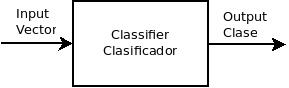
\includegraphics[width=5cm]{diagrams/classifier1.jpg}
\end{center}
\caption{Modelo general de clasificador}
\label{fig:classif1}
\end{figure}

En la figura \ref{fig:classif1} se ve el esquema general de un algoritmo clasificador. Donde lo que se encuentra en la caja ``clasificador'' es el modelo que se va a usar para clasificar. Entonces uno de los problemas que hay que resolver antes de proceder a la clasificación es encontrar un modelo que pueda aproximar lo mejor posible la realidad del problema que se quiere atacar. Varios autores han especificado que hasta el momento no se a encontrado un modelo que se ajuste de la mejor manera a todos los problemas, a esto le han llamado {\it ``no free lunch theorem''}; es español esto traduciría ``teorema no hay almuezo gratis''. En algo si concuerdan la mayoría de investigadores, y es en que si varios modelos funcionan bien se debe escojer el mas sencillo de ellos. Esta observación se desprende del principio filosofico conocido como la navaja de Ockham, propuesto por Guillermo de Ockham (1280-1349), y segun el cual ``cuando dos teorías en igualdad de condiciones tienen las mismas consecuencias, la teoría más simple tiene más probabilidades de ser correcta que la compleja'' \footnote{Robert Audi, ed. Ockham's razor. The Cambridge Dictionary of Philosophy (2nd Edition). Cambridge University Press}. Este principio se aplica en muchos campos, y para el caso del aprendizaje de máquinas tiene especial sentido, ya que usualmente los modelos más sencillos son más fáciles de entrenar, de comprender y sobre todo de depurar.

\subsection{El aprendizaje de máquinas}

Con los avances en las tecnologías de computo, la sociedad tiene la posibilidad de almacenar grandes cantidades de información. Por ejemplo las cadenas de supermercado poseen grandes volumenes de información de sus ventas y las entidades financieras poseen la información crediticia de sus clientes. Para los supermercados es muy útil saber que personas compran ciertos tipos de productos y con que periodicidad, y para las entidades financieras es útil saber que personas son de mayor y menor riesgo para darle un crédito.\newline

Si, por ejemplo, supieramos con exactitud como establecer si una persona es de riesgo o no para una central de crédito dados sus datos financieros, no necesitaríamos utilizar
aprendizaje de máquinas; podríamos simplemente escribir las reglas que determinan si una persona es de riesgo o no en el código. Pero dado que muchas veces no se conocen estas reglas, lo que se busca en el aprendizaje de máquinas es extraer esta información de los datos.\newline

Alpaydin indica que las personas usualmente sabemos que existen procesos que explican los datos que observamos. Por ejemplo, en el caso del supermercado, el comportamiento de los clientes no es completamente aleatorio; por tanto, se espera encontrar algunos patrones en los datos. Aunque este autor indica que muchas veces no es posible identificar el modelo completamente, usualmente se puede construir una buena aproximación. Este es el nicho de trabajo del aprendizaje de máquinas, pues esta aproximación puede ser útil para encontrar patrones en el problema estudiado o para hacer estimaciones de datos futuros asumiendo que en el futuro los datos van a comportarse de una manera similar a como se comportaron en el pasado.

\section{Algunos algoritmos de clasificación}

Como se indicó en la sección anterior, no hay ningun algoritmo que sea la mejor elección para todo tipo de problemas. En esta sección se pretende presentar algunos de los algoritmos o modelos de aprendizaje de máquinas sin ahondar en cada uno de ellos, solo se pretende exponer brevemente de que se tratan y cuales son sus ventajas y desventajas.

\subsection{Árboles de decisión}

Un árbol de decisión es un modelo utilizado principalmente para clasificación. Como su nombre lo dice, el modelo sigue una estructura de árbol, donde los nodos no terminales son condiciones sobre las variables de entrada y los nodos terminales o nodos hoja, son las clases.

\begin{figure}[htb]
\begin{center}
\leavevmode
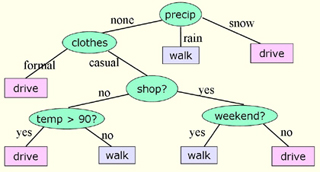
\includegraphics[width=7cm]{img/decisiontree.jpg}
\end{center}
\caption{Ejemplo de árbol de decisión, tomado de MIT OpenCourseware.}
\label{fig:decisionTree}
\end{figure}

En la figura \ref{fig:decisionTree}, se puede ver un ejemplo de un árbol de decisión \footnote{Tomado de ``http://ocw.mit.edu/courses/electrical-engineering-and-computer-science/6-034-artificial-intelligence-spring-2005/'', 12 de Marzo de 2011}. Se puede observar como dependiendo del valor de las variables en cada nodo no terminal, se 
escoje un camino diferente, realizando así un proceso de clasificación. En ese ejemplo, las clases son ``caminar'' y ``conducir''. Es posible examinar el proceso de desición
que se utilizo para llegar a estas variables. Naturalmente, existen procesos automáticos para generar árboles como el del ejemplo a partir de un conjunto de datos de entrenamiento.

De los árboles de decisión se puede concluir:

\begin{itemize}
	\item Son fácilmente interpretables por un ser humano.
	\item Si el árbol esta balanceado correctamente, la velocidad de clasificación es alta.
	\item Se debe configurar la profundidad máxima del árbol.
	\item La mayoría de algoritmos existentes para generar árboles de decisión solo permiten condiciones sobre una única variable por nodo. Por lo tanto el poder clasificatorio de los árboles es limitado.
\end{itemize}

\subsection{Métodos estadísticos}

La estadística es uno de los métodos mas antiguos para inferir el comportamiento de una población a través de una muestra, y sin embargo todavía esta vigente. Se profundizará en este tema en las secciones posteriores, así que por ahora solo se mencionan sus ventajas y desventajas.

\begin{itemize}
	\item No necesita configuración, lo único que se debe saber en el método estadístico a-priori es la distribución de probabilidad con la que se va a  aproximar el modelo real.
	\item El modelo estadístico es fácil de interpretar por un humano, aunque no es tan fácil de intepretar como los árboles de decisión.
	\item El poder clasificatorio es mas alto que el de los árboles de desición.
	\item Brinda mucha información, en vez de solo decir a que clase pertenece una instancia, brida la probabilidad de que la instancia pertenezca a todas las clases, con cierta probabilidad.
\end{itemize}
	
\subsection{Redes neuronales artificiales}

Las redes neuronales artificiales son un paradigma de aprendizaje ampliamente tratado en la literatura de la inteligencia artificial. \footnote{ALPAYDIN, Ethem. Introduction to Machine Learning. Estados Unidos: MIT Press, 2004. 415 p.}. Las redes neuronales artificiales (RNA) intentan imitar la naturaleza de la neuronas del cerebro humano. Uno de los modelos más conocidos de redes neuronales son los perceptrones multicapa. En la figura \ref{fig:rna} se puede apreciar la estructura de un perceptrón multicapa.\footnote{Imagen tomada de Wikimedia Commons ``http://upload.wikimedia.org/wikipedia/commons/6/64/RedNeuronalArtificial.png'', 13 de Marzo de 2011)}.

\begin{figure}[htb]
\begin{center}
\leavevmode
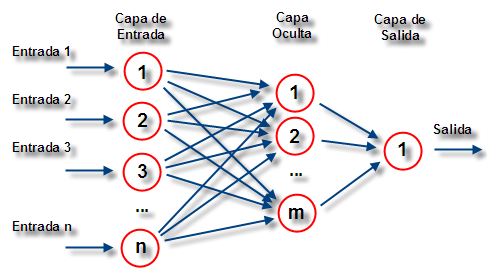
\includegraphics[width=7cm]{img/rna.png}
\end{center}
\caption{Ejemplo de un perceptrón con una capa oculta, tomado de Wikimedia}
\label{fig:rna}
\end{figure}

Cada neurona de un perceptrón multicapa tiene una estructura simple. Cada neurona tiene un vector de datos de entrada $\vec{x}$, un vector de pesos sinápticos $\vec{w}$ y una función de activación $f(x)$. Dado sus entradas, la salida $y$ de una neurona es:

\[y = f(\vec{w}.\vec{x})\]

Las ventajas y desventajas de las redes neuronales son:

\begin{itemize}
	\item El poder clasificatorio de este método es mayor que el de los métodos anteriormente mencionados. Matemáticamente se a demostrado que no exigen ninguna distrubución determinada de los datos, ni separabilidad lineal.
	\item Al igual que el método estadístico, con una función de activación adecuada puede calcular la probabilidad que una instancia pertenezca a cada clase.
	\item Dada la cantidad de parámetros que se pueden configurar, estos algoritmos son muy difíciles de afinar para un problema determinado.
	\item Las redes neuronales son difíciles de interpretar, una vez entrenadas pueden dar buenos o malos resultados, pero es dificil saber cual es el error real o si los resultados se pueden mejorar cambiando los parametros.
\end{itemize}

\section{Algunos elementos de probabilidad}

Un experimento aleatorio es aquel del que no se conoce el resultado con certeza \footnote{Ross, S.M. Introduction to Probability and Statistics for Engineers and Scientists. New York: Wiley 1987.}. El conjunto de todos los posibles resultados se llama espacio muestral $S$, y a cualquier subconjunto de $S$ se le llama evento $E$. Se puede interpretar la probabilidad como una frecuencia: cuando un experimiento es repetido continuamente bajo las mismas condiciones, la proporción de veces que ocurre el evento $E$ en el tiempo se aproxima a un valor constante; a esto lo denotamos $P(E)$ e indica la probabilidad que el evento $E$ ocurra. De igual manera, una variable aleatoria es aquella que puede tomar cualquier valor en distintos experimentos, es decir, su valor no se puede determinar con certeza.

\subsection{Probabilidad condicional y el teorema de Bayes}

La probabilidad condicional es la probabilidad de que un evento $A$ ocurra, dado que se conoce la ocurrencia del evento $B$, y se denota $P(A|B)$. La probabilidad condicional se calcula como:

	\begin{equation}\label{eq:condProb}
		P(A|B) = \frac{P(A \cap B)}{P(B)}
	\end{equation}

Al saber que ocurrió el evento $B$, el espacio muestral se reduce al subconjunto $B$. Dado que la intersección es conmutativa, de la equación \ref{eq:condProb} se obtiene:

\[P(A \cap B) = P(A|B)P(B) = P(B|A)P(A)\]

Y con esto se llega al teorema de Bayes:

	\begin{equation}\label{eq:bayes}
		P(A|B) = \frac{P(B|A)P(A)}{P(B)}
	\end{equation}

Cuando el espacio muestral se compone de varios eventos mutuamente exclusivos $A_i$, es decir, $\cup_{i=1}^{n} A_i = S$ entonces:

\[P(B)=\cup_{i=1}^{n} {A_i \cap B}\]
	\begin{equation}\label{eq:bayesDenominator}
		P(B) = \sum_{i=1}^{n}{P(B|A_i)P(A_i)}
	\end{equation}

Entonces, reemplazando Eq.\ref{eq:bayesDenominator} en Eq.\ref{eq:bayes}, tenemos:
	
	\begin{equation}\label{eq:bayes2}
		P(A|B) = \frac{P(B|A)P(A)}{\sum_{i=1}^{n}{P(B|A_i)P(A_i)}}
	\end{equation}
	
\subsection{La esperanza matemática}

Supongamos que se realiza un experimento sobre una variable aleatoria $x$ un número infinito de veces, entonces la esperanza de la variable $x$ es el promedio del valor de $x$ en los infinitos experimentos y se denota $E[x]$ (que se lee valor esperado de $x$ o esperanza). El concepto de esperanza es importante en la probabilidad porque además de tener usualmente un significado de interés en la variable aleatoria estudiada, se espera que independiente de la distribución de probabilidad que sigue la variable $x$, la esperanza de $x$ converge a un valor constante si las condiciones del experimento no cambian. Matematicamente el valor de la esperanza de una variable aleatoria $x$ es el siguiente:

	\[ E(X) = \left\{ \begin{array}{ll}
		\sum_{i}{x_iP(x_i)}   & \mbox{si X es una variable discreta} \\
		\int {xp(x)dx} & \mbox{si X es una variable continua}
	\end{array} \right. \]

La esperanza es entonces un promedio ponderado, en donde el peso de cada valor tomado es la probabilidad de que la variable X tome dicho valor. Suponiendo que $X$ y $Y$ son dos variables aleatorias, la esperanza cumpla las siguientes propiedades:

	\[E[aX + b] = aE[X] + b\]
	\[E[X + Y] = E[X] + E[Y]\]

La esperanza de toda función g para la cual $imagen(g) \in \Re$ es:

	\[ E[g(X)] = \left\{ \begin{array}{ll}
		\sum_{i}{g(x_i)P(x_i)}   & \mbox{si X es una variable discreta} \\
		\int {g(x)p(x)dx} & \mbox{si X es una variable continua}
	\end{array} \right. \]

Una función especial se da cuando $g(X) = x^n$:

	\[ E[X^n] = \left\{ \begin{array}{ll}
		\sum_{i}{x_i^nP(x_i)}   & \mbox{si X es una variable discreta} \\
		\int {x^np(x)dx} & \mbox{si X es una variable continua}
	\end{array} \right. \]

Esta función se denomina el enésimo momento de X. El primer momento, por ejemplo, es la media.

\subsection{Desviación estandar, varianza y covarianza}

La varianza mide que tanto varia X alrededor de el valor esperado, si X es una variable aleatoria entonces la varianza se define como el segundo momento menos el cuadrado del primer momento:

	\[Var(X) = E[X^2] - E[X]^2 = E[X^2] - \mu^2\]

La desviación estandar es la raiz cuadrada de la varianza, y como se expresa en las mismas unidades de X entonces es más utilizada que la varianza, pues puede ser interpretada de una manera más facil. La desviación estandar se denota usualmente con el simbolo $\sigma$.

La covarianza indica la relación que existe entre dos variables aleatorias X y Y. Si la ocurrencia de X hace más probable la ocurrencia de Y, entonces la covarianza es positiva. Si por el contrario la ocurrencia de X hace menos probable la ocurrencia de Y, entonces la covarianza es negativa. Si las dos variables no estan relacionadas, entonces la covarianza sera 0. La covarianza se define matematicamente como:

	\[Cov(X, Y) = E[XY] - \mu_X\mu_Y\]


\subsection{Distribución de probabilidad}

Una distribución de probabilidad de una variable aleatoria X es una función que asigna una probabilidad a cada posible valor que puede tomar la variable X. Cuando X es una variable discreta, la función definira un valor de probabilidad para cada uno de los valores que puede tomar, sin embargo, cuando la variable X es continua, existen infinitos valores posible que puede tomar y por tanto la probabilidad de obtener un valor especifico es 0. Por esta razón tiene poco sentido hablar de la probabilidad de un valor especifico y la distribución de probabilidad se convierte en una función de distribución, la cual define, para cada real x, la probabilidad de que la variable X sea menor o igual a x. En esto caso la distribución de probabilidad D se definiría matematicamente como:

	\[D(x) = P(X \leq x) = \int_{-\infty}^x{f(t)dt}\]

Donde f(t) es una función de densidad continua, que debe ser positiva para todo t, y que debe cumplir la propiedad:

	\[\int_{-\infty}^{\infty}{f(t)dt} = 1\]
	
\subsection{La distribución normal}

Muchos elementos de la naturaleza obedecen a una distribución normal, al menos de manera aproximada. Esta distribución tiene forma de campana, que significa que los datos se obtienen al rededor de un valor típico con ligeras variaciones. Matemáticamente, si $\mu$ representa el valor típico y $\sigma$ representa cuanto varían las instancias al rededor de este valor típico, la distribución está dada por:
\begin{equation}
	p(x) = \frac{1}{\sqrt{2\pi}\sigma}exp\left[-\frac{(x-\mu)^2}{2\sigma^2}\right]
	\label{eq:normal}
\end{equation}
Donde $exp[x]$ es la función exponencial $e^x$, $\mu$ son la media y $\sigma$ se conoce como desviación estandar, que se calculan como se especifica en las secciones anteriores. El 68.27\% de los datos está entre $(\mu-\sigma, \mu+\sigma)$, el 95.45\% de los datos está entre $(\mu-2\sigma, \mu+2\sigma)$ y el 99.73\% de los datos está entre $(\mu-3\sigma, \mu+3\sigma)$.


\section{La distribución normal multivariable}
\label{sect:multivar}

En muchas ocaciones, en lugar de calcular un único valor $x$ de cada elemento muestreado, se calculan varios valores diferentes generando un vector $\vec{x}$. Supongamos que tenemos un vector d-dimensional $\vec{x}$ que sigue una distribución normal multivariable, entonces:
	\begin{equation}\label{eq:multDens}
		p(x) = \frac{1}{(2\pi)^{d/2}|\Sigma|^\frac{1}{2}} exp\left[{-\frac{1}{2}(\vec{x}-\vec{\mu})\Sigma^{-1}(\vec{x}-\vec{\mu})}\right]
	\end{equation}
Esto se denota como $\vec{x} \sim N(\vec{\mu},\Sigma)$ y significa que $\vec{x}$ sigue una distrubución normal multivariable cuya media es el vector $\vec{\mu}$ y cuya matriz de covarianza es la matriz $\Sigma$. Si para cada clase $C_i$ se calculan la media $\vec{\mu_i}$ y la matriz de covarianza $\Sigma_i$, la densidad de probabilidad $p(x|C_i)$ es:
	\begin{equation}\label{eq:multivariate}
		p(x|C_i) = \frac{1}{(2\pi)^{d/2}|\Sigma_i|^\frac{1}{2}} exp\left[{-\frac{1}{2}(\vec{x}-\vec{\mu_i})\Sigma_i^{-1}(\vec{x}-\vec{\mu_i})}\right]
	\end{equation}
	
La distribución normal multivariable puede ser utilizada como un algoritmo de clasificación, y este modelo ha demostrado ser robusto para varias aplicaciones diferentes\footnote{Jerome H. Friedman. Regularized discriminant analysis. Journal of the american statistical association, 84:165–175, 1989.}.	El objetivo de este modelo es encontrar $P(C_i|x)$,	que es la probabilidad posterior de que el vector $\vec{x}$ pertenezca a la clase $C_i$. Si se calcula $P(C_i|x)$ para cada clase $i$, se escoje como la clase correcta la que poseea la probabilidad posterior mas alta. \newline \newline
Es importante notar que en lugar de simplemente determinar a que clase pertenece la instancia dada, se estan calculando también las probabilidades que representan la seguridad con la que el algoritmo está concluyendo su respuesta. Esto es una ventaja para el problema de reconocimiento óptico de caracteres, ya que algunas correcciones pueden realizarse en etapas posteriores, por ejemplo, usando un diccionario. \newline \newline
Como se muestra en la ecuación \eqref{eq:multivariate}, lo que permite calcular la distribución normal multivariable es $p(x|C_i)$, que es la desidad de probabilidad de la variable aleatoria $\vec{x}$ dada la clase $C_i$; lo que se desea calcular en cambio es la probabilidad de que un $\vec{x}$ dado pertenezca a la clase $C_i$, es decir, la probabilidad posterior $P(C_i|\vec{x})$. Para eso se usa el teorema de Bayes (Ecuación \ref{eq:bayes2}). Entonces la probabilidad posterior se calcula como:
	\begin{equation}\label{eq:multBayes}
		P(C_i|\vec{x}) = \frac{p(\vec{x}|C_i)P(C_i)}{p(x)} = \frac{p(\vec{x}|C_i)P(C_i)}{ \sum_j{p(\vec{x}|C_j)P(C_j)} }
	\end{equation}
	
De la ecuación \ref{eq:multBayes} se puede ver inmediatamente que $\sum_i{P(C_i|\vec{x})}=1$, y que $0 \le P(C_i|\vec{x}) \le 1$ para todas las clases.
	
\subsection{Entrenamiento}

Ya se ha visto como se puede llevar a cabo la clasificación una vez que los parámetros $\vec{\mu_i}$ y $\Sigma_i$ han sido calculados para cada clase $C_i$. Entonces el entrenamiento consiste en calcular los parámetros $\vec{\mu_i}$ y $\Sigma_i$ a partir de un conjunto de entrenamiento $T$. Primero, el conjunto de entrenamiento debe ser partido en diferentes conjuntos de entrenamiento $T_i$, donde cada conjunto $T_i$ contiene solamente instancias cuya clase es $C_i$. Entonces, los parámetros se calculan con las ecuaciones \ref{eq:multiParams}.
\begin{equation}\label{eq:multiParams}
\begin{aligned}
	\vec{\mu_i} &= E[ \vec{x_i} ] \\
	\Sigma_i(a,b) &= E[ (\vec{x_i}-\vec{\mu_a})(\vec{x_i}-\vec{\mu_b}) ]
\end{aligned}
\end{equation}
Donde $\vec{x_i}$ son las instancias del conjunto $T_i$, $E[x]$ es el valor esperado o media de $x$ y $\Sigma_i(a,b)$ es el valor en la fila $a$ y la columna $b$ de la matriz $\Sigma_i$.

\subsection{Simplificaciones de la distribución normal multivariable}

El número de parámetros de la distribución normal multivariable crece cuadráticamente con el número de dimensiones d, dado que la matriz de covarianza es de tamaño $d \times d$. Esto se convierte en un problema cuando no hay suficientes datos para estimar los parámetros de manera apropiada \footnote{Wald and Kornmal. Discriminant functions when covariances are unequal and sample sizes are moderate. Biometrics, 33:479–484, 1977.}. Supongamos que de una muestra de trés instancias se desea calcular la media y la varianza de la población; Es claro que aunque los parámetros pueden ser calculados, probablemente no representarán bien los parámetros de la población. De la misma manera, cuanto mas parámetros se deban calcular se necesitan mas datos para una mejor generalización.\newline \newline
Entonces, algunas veces es deseable reducir la cantidad de parámetros para obtener una mejor generalización. En el caso de una distribución normal multivariable, un enfoque para simplificar el modelo es usar una matriz de covarianza compartida por todas las clases. Las probabilidades posteriores pueden ser calculadas de la misma manera, y se sigue escojiendo la clase con mayor probabilidad posterior. Esto es equivalente a calcular la distancia Mahalanobis entre la entrada y la media de cada clase y escojer la que tenga la menor distancia. La distancia Mahalanobis $d_i$ entre la entrada $\vec{x}$ y la clase $C_i$, esta dada por:
\begin{equation}
\label{eq:mahalanobis}
 d_i = (\vec{x}-\vec{\mu_i})\Sigma(\vec{x}-\vec{\mu_i}) 
\end{equation}
Note que cuando la matriz de covarianza es igual a la matriz identidad, la distancia Mahalanobis se convierte en la distancia Euclidiana al cuadrado.\newline \newline
Una mezcla entre el método completo de distribución normal multivariable y el modelo con matriz de covarianza compartida puede dar buenos resultados cuando hay riezgo que el determinante de la matriz de covarianza sea muy cercano a cero. A este método se le denominará una distribución normal multivariable con matriz de covarianza semi-compartida. Que se definiría por la ecuación:
\begin{equation}\label{eq:semishared}
	p(x|C_i) = \frac{1}{(2\pi)^{d/2}|\Sigma|^\frac{1}{2}} e^{-\frac{1}{2}(\vec{x}-\vec{\mu_i})\Sigma_i^{-1}(\vec{x}-\vec{\mu_i})}
\end{equation}
Donde todas las variables tienen el mismo significado que el la ecuación Eq.\ref{eq:multivariate}. Note que la única diferencia entre Eq.\ref{eq:multivariate} y Eq.\ref{eq:semishared} es que la matriz de covarianza en el coeficiente es compartida para todas las clases $\Sigma$; pero la matriz de covarianza en el exponente $\Sigma_i$ sigue siendo diferente para todas las clases (No es compartida).	
	

\chapter{Extracción de características de los caracteres}
\label{chap:features}

\section{Escala de grises}

Antes de computar los momentos invariantes es necesario hacer un preprocesamiento. Primero la imagen debe convertirse a un formato más apropiado para extraerle las caracteristicas. Dado que las letras no varian con el color, y que el objetivo del sistema no es reconocer colores, es conveniente convertir la imagen a una escala de grises. En este proyecto se trabajo con el modelo RGB. En este modelo se asigna una intensidad a cada uno de los tres colores primarios de la luz: rojo, verde y azul\footnote{que en ingles son red, green, y blue, de alli las iniciales RGB}, de esta manera cada pixel en una fotografia se representa mediante un valor que identifique la intensidad de cada uno de estos tres colores que, mezclados por adición, se acerque más al color verdadero del pixel. Las camaras digitales modernas utilizan valores entre\footnote{en donde 0 representa que el color no se utiliza y 255 representa la mayor intensidad} 0 y 255 ($2^8$) permitiendo de esta manera más de 16 millones de colores distintos. En una escala de grises, en cambio, cada pixel es representado con un unico valor entre 0 y 255, el cual representa que tan oscuro es el mismo. Para convertir un pixel de una imagen en color a uno en escala de grises se suele hacer un promedio ponderado de la intensidad de cada uno de los tres colores, en donde a cada color se le asigna un peso. Al ser un promedio ponderado la suma de los tres pesos debe ser 1. Los pesos utilizados más comunmente son:

\begin{equation}\label{bwtocv}
	gris = 0.2989 * rojo + 0.5870 * verde + 0.1140 * azul 
\end{equation}

Estos pesos son usados por la libreria de visión computador OpenCV\footnote{$http://opencv.willowgarage.com/documentation/c/miscellaneous_image_transformations.html$} y fueron calculados a partir de observaciones de la sensibilidad del ojo humano a cada uno de los tres colores. 

Utilizando la ecuación \eqref{bwtocv} se escribio un algoritmo para obtener una imagen en escala de grises a partir de una imagen RGB. 

\section{Binarización}

Una vez obtenida la imagen escala de grises se procedio a hacer una binarización. La binarización es un proceso que transforma una imagen en escala de grises a una imagen en dos colores: blanco o negro. Esto es util para el reconocimiento de caracteres debido a que las letras y los digitos en escala de grises no se distinguen por la intensidad de los pixeles que los componen sino por la forma que estos producen. De esta forma, al convertir las imagenes a blanco y negro se pierde muy poca información relevante y se simplifica la representación de cada pixel, pasando de 256 posibles valores a tan solo 2. Un metodo muy utilizado para binarizar una imagen es escoger un valor umbral $T(x,y)$ para cada pixel $(x,y)$ y establecer el valor del pixel como:

\begin{equation}\label{binEq}
 I_2(x,y) = \left\{ \begin{array}{ll}
	0   & \mbox{si $I_1(x,y) < T(x,y)$} \\
	255 & \mbox{en cualquier otro caso}
\end{array} \right. 
\end{equation}

Donde $I_1(x,y)$ es la imagen original y $I_2(x,y)$ es la imagen binarizada. Usualmente, la diferencia entre los distintos metodos de binarización se encuentra en como elige cada uno el umbral $T(x,y)$.\newline
Cuando las imagenes son adquiridas mediante un escaner, es común escoger un $T(x,y)$ constante para todos los pixeles. Esto es debido a que los escaners logran una iluminación aproximadamente constante en todo el documento. Como en este caso la imagen es tomada por una camara digital, en condiciones de ilumnación no tan constantes, se eligio un metodo de binarización basado en el método local del valor umbral. En este metodo $T(x,y)$ puede ser distinto para distintos pixeles, y se dice que es local porque $T(x,y)$ se calcula utilizando información sobre el vecindario de pixeles del pixel $(x,y)$. El metodo que ha dado\footnote{Efficient Implementation of Local Adaptive Thresholding Techniques Using Integral Images} los mejores resultados para el reconocimiento de caracteres es el de Sauvola, en el cual $T(x,y)$ se obtiene utilizando la siguiente ecuación:

\begin{equation}
      T(x,y)=m(x,y)\left[ 1 + k(\frac{s(x,y)}{R}-1) \right]
\end{equation}

Donde $m(x,y)$ es la media y $s(x,y)$ la desviación estandar de los pixeles en algun area alrededor de X, y R es el maximo valor de la desviación estandar (128 para una imagen en escala de grises). La forma más sencilla de implementar este algoritmo es calcular para cada pixel $(x,y)$ el valor de $m$ y $s$ de manera directa, es decir, iterar por todos los pixeles en el vecindario de $(x,y)$. Sin embargo, si el area a considerar para $m$ y $s$ es de tamaño $O \times O$, entonces la complejidad computacional de calcular $T(x,y)$ para todos los pixeles de una imagen de tamaño $N \times M$ seria $O(N \times M \times O^{2})$. Con esta complejidad el algoritmo seria demasiado lento para procesar imagenes de varios megapixeles, incluso con valores relativamente pequeños de $O$.

\subsection{Optimización al algoritmo al algoritmo de binarización}

\section{Componentes conectados}

\section{Extracción de caracteristicas}

Como se explicó en el capítulo \ref{chap:ml}, los métodos de clasificación necesitan unas características de entrada que permitan diferenciar los objetos a clasificar. En el caso específico de los métodos estadísticos, se necesitan vectores de números reales que sean similares para el mismo caracter independiente de el tamaño o inclinación que tenga en caracter en cuestión. Si las imagenes fueran adquiridas mediante un escaner, la inclinación podria ser muy pequeña, incluso tanto que podria despreciarse. Sin embargo, cuando las imagenes son adquiridas mediante una camara digital, la inclinación entra a ser un factor importante, más aun cuando quien las obtiene es una persona invidente. Por estas razones  se deben buscar características que sean invariantes a la rotación y al escalamiento, es decir, que al rotar o escalar un mismo caracter el valor numérico de las caracteríticas sea similar. Dado que la entrada del método estadístico en un vector, esta similitud se puede expresar en terminos vectoriales como que debe existir una distancia Mahalanobis (Eq. \ref{eq:mahalanobis}) relativamente pequeña entre el vector de características de la imagen original y de la imagen rotada.

Para lograr un cierto grado de independencia de las características a la rotación y al escalamiento se muestran dos enfoques: un primer enfoque es transformar la imagen, esto significa rotarla y escalarla para hacerla lo mas similar posible a un patrón estandar, despues de esto se extraerian de la misma caracteristicas que sean dependientes a la rotación y el escalamiento. Un segundo enfoque consiste en trabajar la imagen tal cual es tomada por la cámara, y utilizar características matemáticas en las que se obtengan valores numéricos similares para una misma imagen rotada y escalada, es decir, que sean invariantes a la rotación y el escalamiento. En las secciones posteriores se presentan ambos enfoques junto con sus ventajas y desventajas.

\subsection{Rotación y escalamiento mediante transformación geometrica}

Si se utilizan caracteristicas dependientes a la rotación, se debe entrenar el clasificador con distintas instancias que tengan distintos angulos de rotación. Si se hace dificil obtener ejemplos reales, una opción puede ser construir ejemplos virtuales \cite{niyogi2002}. El problema con este enfoque es que cada caracter se convertiria en muchos clases distintas, cada una de las cuales tendria un angulo de rotación. Asi pues, el numero de clases aumentaria significativamente, y aun asi, todas las rotaciones de una misma letra serian en realidad parte de una sola clase. Como resultado de lo anterior, no solo aumentaria la complejidad computacional del algoritmo de clasificación, sino que ademas disminuiria la probabilidad de que este clasificara correctamente, por cuanto el numero de clases seria de varios miles.

Un enfoque mucho más practico es detectar la rotación y el escalamiento del texto, y posteriormente aplicar transformaciones geometricas para ajustar la rotación y el escalamiento a valores preestablecidos. Posteriormente se podrian obtener caracteristicas dependientes a la rotación y el escalamiento para clasificar cada letra. Para detectar la rotación se pueden utilizar metodos ya existentes, como los utilizados en el algoritmo de analisis de documentos Docstrum, los cuales permiten establecer cual es la inclinación de cada linea de texto. Al tener la inclinación de las lineas, se puede determinar cual es la inclinación da cada caracter en particular. Para corregir la inclinación se utilizaria una matriz de rotación: si el algoritmo de detección de rotación determina que el caracter esta rotado un angulo $\theta$ alrededor de su centroide, se puede detectar cual es la nueva ubicación $(x', y')$ del pixel $(x, y)$ utilizando la siguiente operación:

	\[
		\begin{pmatrix} 
			x' \\ y'
		\end{pmatrix}
		=
		\begin{pmatrix} 
			\cos\theta & -\sin\theta \\
			\sin\theta & \cos\theta
		\end{pmatrix}
		\begin{pmatrix} 
			x \\ y
		\end{pmatrix}
	\]


El escalamiento se podria ajustar haciendo una interpolación de los pixeles al tamaño deseado. Existen, sin embargo, dos problemas con esta solución. En cuanto a la rotación, si el angulo $\theta$ no es un multiplo de 90 grados, las coordenadas de los nuevos pixeles $(x', y')$ no serian enteras. Esto se puede solucionar interpolando $(x',y')$ a sus vecinos enteros más cercanos, pero este proceso conlleva una perdida de información importante cuando la calidad de las imagenes no es muy buena. En cuanto al escalamiento, la interpolación tambien produce una perdida de información. Ambos problemas podrian ocasionar que la imagen obtenida finalmente fuese muy distinta a la imagen original, lo que haria el proceso de clasificación mucho más dificil.

Dado que los algoritmos de clasificación funcionan de la mejor manera cuando tienen la mayor cantidad de información util, es convinente encontrar metodos de extracción de caracteristicas que minimizen la perdida de información. Una posibilidad es utilizar caracteristicas que sean invariantes a la rotación y al escalamiento, pues de esta forma no es necesario rotar o escalar la imagen. Los momento invariantes son caracteristicas que cumplen dicha propiedad.

\subsection{Momentos invariantes de Hu}	
\label{sect:invariants}

Los momentos invariantes fueron propuestos por primera vez por Hu\cite{Hu62}. Estos momentos pueden ser considerados como un promedio ponderado de los pixeles de una imagen. Hu computo sus invariantes utilizando los momentos geometricos, los cuales son variantes a la rotación y al escalamiento. Los momentos geometricos se definen como:

	\begin{equation}\label{eq1}
		\mu_{pq} = \iint{ {(x-\bar{x})^p} {(y-\bar{y})^q} f(x,y) dy dx }
	\end{equation}

Donde $\mu_{pq}$ es el momento geometrico de orden $(p+q)$, $f(x,y)$ es el valor del pixel en la posición $(x,y)$ de la imagen y $(\bar{x},\bar{y})$ es el centroide de la misma. Partiendo de estos momentos podemos obtener $n_{pq}$, un momento de orden $(p+q)$ que es invariante al escalamiento:

	\begin{equation}\label{eq2}
		n_{pq} = \frac{\mu_{pq}}{ \mu_{00}^{1+\frac{p+q}{2}} }
	\end{equation}

Utilizando $n_{pq}$, Hu logro un conjunto de momentos invariantes, todos con un grado menor o igual a 3. Sus siete momentos invariantes son:

	\begin{align*}
		\phi_1 =& n_{20} + n_{02},\\
		\phi_2 =& (n_{20} - n_{02})^{2} + 4n_{11}^{2},\\
		\phi_3 =& (n_{30} - 3n_{12})^{2} + (3n_{21} - n_{03})^{2},\\
		\phi_4 =& (n_{30} + n_{12})^{2} + (n_{21} + n_{03})^{2},\\
		\phi_5 =& (n_{30} - 3n_{12})(n_{30} + n_{12})((n_{30} + n_{12})^{2}\\
				& - 3(n_{21} + n_{03})^{2}) + (3n_{21} - n_{03})(n_{21} + n_{03})\\
				& \times (3(n_{30} + n_{12})^{2} - (n_{21} + n_{03})^{2}),\\
		\phi_6 =& (n_{20} - n_{02})((n_{30} + n_{12})^{2} - (n_{21} + n_{03})^{2})\\
				& + 4n_{11}(n_{30} + n_{12})(n_{21} + n_{03}),\\
		\phi_7 =& (3n_{21} - n_{03})(n_{30} + n_{12})((n_{30} + n_{12})^{2}\\
				& - 3(n_{21} + n_{03})^{2}) - (n_{30} - 3n_{12})(n_{21} + n_{03})\\
				& \times (3(n_{30} + n_{12})^{2} - (n_{21} + n_{03})^{2})\\
	\end{align*}

\subsection{Momentos complejos y momento de Fluzzer}

En 1984 Mostafa y Psaltis \cite{mostaf84} propusieron los momentos complejos como una forma alternativa de lograr momentos invariantes. Un momento complejo $C_{pq}$ de orden $(p+q)$ para una imagen $f(x,y)$ se define como:

	\[ C_{pq} = \iint{ (x+iy)^p (x-iy)^q f(x,y) dx dy } \]
	
Donde i denota la unidad imaginaria. En coordenadas polares esto es equivalente a:

	\begin{equation}\label{polarCplx}
		C_{pq} = \iint{ r^{p+q+1}e^{i(p-q)\theta}f(r,\theta) dr d\theta }
	\end{equation}

Una propiedad interesante de los momentos complejos, que se deriva de la ecuación \eqref{polarCplx}, es que, si hay una imagen $f'(r,\theta)$ que es una versión rotada un angulo de $\alpha$ sobre el origen de la imagen $f(r,\theta)$\footnote{es decir $f'(r,\theta) = f(r,\theta+\alpha)$} entonces:

\begin{equation}\label{rotProp}
	C'_{pq} = e^{-i(p-q)\alpha}C_{pq}
\end{equation}

Donde $C'_{pq}$ es el momento complejo de $f'(r,\theta)$ y $C_{pq}$ es el momento complejo de $f(r,\theta)$. Flusser noto \cite{flusser99} que aun cuando se puede probar de la equación \eqref{rotProp} que $|C_{pq}|$ es invariable a la rotación, estos momentos no generan un conjunto completo de invariantes. Flusser tambien demostro que los momentos de Hu no eran ni completos ni independientes, y propuso un metodo para generar un conjunto completo de momentos invariantes de orden arbitrario. Cuando este metodo se utiliza para generar momentos de grado menor o igual a cuatro, se obtienen 11 momentos invariantes.

\subsection{Corrección de la rotación}

\subsection{Problemas de simetria}

Sin embargo, en un articulo diferente\cite{flusser06} Flusser demostro que muchos de estos momentos son iguales a cero cuando los objetos que se intentan reconocer con ellos tienen algun grado de simetria y, para solucionar este problema, propuso un nuevo metodo para generar momentos adecuados para reconocer objetos con simetria de grado N. Como se mostrara mas adelante estos momentos son tambien efectivos para reconocer objetos que no son simetricos.

\subsubsection{Correción de los problemas de simetria}

\chapter{Diseño, implementación y pruebas del aplicativo}
\label{chap:ingSw}

 %aquí comienza la burocracia
\section{Análisis}
La primera etapa en el desarrollo de software es la de levantamiento de requerimientos. Los requerimientos se toman de los objetivos de desarrollo del proyecto(Ver sección \ref{sect:objective}). Los objetivos muestran que se requiere desarrollar una aplicación para reconocimiento de dígitos usando para clasificar el modelo estadístico multivariable explicado en la sección \ref{sect:multivar} y para la extracción de características los momentos invariantes explicados en la sección \ref{sect:invariants}.\newline \newline
Se detectó que la aplicación se puede modelar usando dos casos de uso, ya que desde el punto de vista de los actores solo hay dos funciones que pueden desempeñar con la aplicación. El diagrama se muestra en la Figura \ref{fig:useCase}. Un caso de uso, desempeñado por un usuario administrador, es el del entrenamiento del modelo. El otro caso de uso, desempeñado por el usuario final, es el de reconocimiento de caracteres en el documento fotografiado.

\begin{figure}[htb]
\begin{center}
\leavevmode
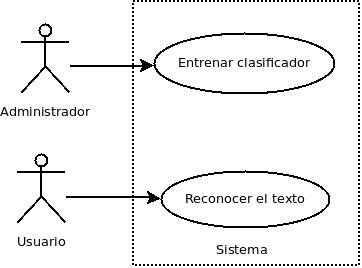
\includegraphics[width=7cm]{diagrams/casoUso.jpg}
\end{center}
\caption{Diagrama de casos de uso}
\label{fig:useCase}
\end{figure}

\subsection{Documentación de casos de uso}
La documentación de los casos de uso se ven respectivamente en la tabla \ref{tb:uc1} y la tabla \ref{tb:uc2}.

\begin{table}
\begin{center}
\begin{tabular}{|p{5cm}|p{5cm}|}
	\hline
	Caso de uso & Entrenamiento del sistema de clasificación\\
	\hline
	Actor: Usuario administrador & Referencia: 1 \\
	\hline
	Precondición: Sistema no entrenado. Imagenes de entrenamiento en un mismo directorio nombradas como se explica en la sección \ref{sect:testEnvironment} & 
	Postcondición: Sistema entrenado. \\
	\hline
	Sistema & Usuario \\
	\hline
	1. El usuario administrador indica en que directorio se encuentran las imagenes de entrenamiento. &
	2. El sistema construye un conjunto de entrenamiento como se explica en la sección \ref{sect:trainingSet} con todas las imágenes del directorio pasado por el usuario. \\
	\hline
	4. El usuario recibe un mensaje que indica que el procedimiento se realizó con éxito. &
	3. El sistema se entrena como se explica en el capítulo \ref{chap:ml} y guarda el modelo en disco. \\
	\hline
\end{tabular}
\end{center}
\caption{Caso de uso 1}	
\label{tb:uc1}
\end{table}

\begin{table}
\begin{center}
\begin{tabular}{|p{5cm}|p{5cm}|}
	\hline
	Caso de uso & Entrenamiento del sistema de clasificación\\
	\hline
	Actor: Usuario final & Referencia: 2 \\
	\hline
	Precondición: Sistema entrenado & Postcondición: El usuario tiene el texto solicitado. \\
	\hline
	Sistema & Usuario \\
	\hline
	1. El usuario le envía al sistema una imagen del documento que desea leer. Las condiciones de captura de la imagen deben estar entre las especificadas en la sección \ref{sect:population}. &
	2. El sistema binariza la imagen, la segmenta y reconoce los caracteres segmentados en la imagen. \\
	\hline
	4. El usuario recibe el texto reconocido por el sistema &
	3. El sistema envía al usuario el texto reconocido de la imagen enviada. \\
	\hline
\end{tabular}
\end{center}
\caption{Caso de uso 2}	
\label{tb:uc2}
\end{table}

\section{Diseño}
El diseño del aplicativo se realizó con los diagramas de secuencia y clases de el estandar UML.

\chapter{Metodología de la investigación}
\label{chap:metodology}

\section{Diseño metodológico}
	\subsection{Hipótesis}
	Es posible desarrollar un sistema de reconocimiento óptico de dígitos usando el teorema de Bayes con una distribución normal multivariable y tomando como características los momentos invariantes de Hu y de Fluzzer al procesar una imagen de un documento que cumpla con las restricciones establecidas (Ver población), tomando la imagen con	una cámara de un celular inteligente y ejecutando el programa en un sistema de cómputo.
		
	\subsection{Tipo de investigación}
	En esta investigación se utilizará un enfoque cuantitativo.
	
	\subsection{Población}
	\label{sect:population}
	Los documentos impresos que solo contengan dígitos numéricos, que cumplan con las siguientes restricciones:
	\begin{itemize}
	\item Forma rectangular.
	\item Fondo blanco.
	\item Letra de color negro y con un único tipo de letra o fuente.
	\item El tamaño de los dígitos varía entre 12 y 20 puntos
	\item La inclinación de los dígitos varía entre -30$^{\circ}$ y 30$^{\circ}$.
	\end{itemize}
	
	\subsection{Unidad de análisis}
	Fotos de textos con las condiciones mencionadas en la población, con una única fuente.

	\subsection{Muestra}
	Se tomará una muestra de 10 páginas, una página por cada dígito. Cada página contendrá entre 100 y 120 instancias de cada dígito con una única fuente pero con diferentes tamaños de letra en el rango especificado. De cada página se tomarán 5 fotos con diferentes inclinaciones en el rango de inclinación especificado. Las fotos deben ser tomadas desde un punto perpendicular al papel. De todo el conjunto de instancias recolectadas, se seleccionará aleatoriamente un 70\% de los datos para el conjunto de entrenamiento, un 15\% para el conjunto de validación otro 15\% para el conjunto de pruebas. Los datos se dividen para verificar la capacidad de generalización del método de aprendizaje, sobre datos que no se le mostraron en el entrenamiento.
	
	\subsection{Variables}
	Las variables a tener en cuenta para ejecución de la aplicación son:
	\begin{itemize}
	\item Porcentaje de caracteres reconocidos exitosamente en total.
	\item Porcentaje de caracteres reconocidos exitosamente por cada dígito.
	\item Porcentaje de seguridad con el que se reconocieron los dígitos en total.
	\item Porcentaje de seguridad con el que se reconoció cada dígito.
	\item Latencia (Tiempo que se demora el OCR en comenzar a entregar salida)
	\end{itemize}

\section{Escenario de pruebas}
\label{sect:testEnvironment}
En esta sección se pretende ilustrar cual fue la metodología seguida para las pruebas y las condiciones bajo las que se tomaron los datos. Cabe anotar que para realizar las mediciones se debe contar con un conjunto de datos de entrenamiento y un conjunto de datos de validación, ya que como se explicó en el capítulo \ref{chap:ml}, primero se debe crear el modelo con los datos de entrenamiento y luego se debe probar la habilidad de generalización sobre un conjunto de datos no usado para el entrenamiento.

\subsection{Levantamiento de datos}
Se entiende por un conjunto de datos de entrada etiquetado, un conjunto de datos de entrada en el que de cada dato de entrada se conoce la clase a la que pertenece. Asi que tanto el conjunto de entrenamiento $T$ como el conjunto de validación $V$ deben ser conjuntos etiquetados.\newline \newline
La forma mas fácil de construir estos dos conjuntos, es construir un único conjunto etiquetado $S$ y luego dividirlo aleatoriamente en los dos conjuntos $T$ y $V$. Tal que los conjuntos $T$ y $V$ sean disjuntos, es decir, que $T \cap V = \emptyset$ y $T \cup V = S$ donde $\emptyset$ representa el conjunto vacío.\newline\newline
Para construir el conjunto de datos etiquetados $S$ se siguió el siguiente procedimiento:
\begin{itemize}
	\item Se imprimió una hoja por cada símbolo a reconocer. Cada hoja contenía entre 350 y 450 instancias del mismo símbolo, con tamaño de fuente variando entre 12 puntos y 20 puntos, pero todos los símbolos fueron impresos con el mismo tipo de letra o fuente.
	\item Por cada página se tomaron 5 fotos con una cámara digital de 4 megapixeles. En cada foto se variaba ligeramente la distancia de la que se tomaba la foto para incluir mas variabilidad en la escala de las imágenes. También se variaba el ángulo de inclinación del texto en ángulos entre $-30^\circ$ y $30^\circ$.
	\item A cada imagen se le dió un nombre que le permitiera saber al sistema que símbolos se encuentran en esa foto. Todas las imagenes de números, tienen un nombre de la forma \verb/t<num>_<consec>.jpg/, donde \verb/<num>/ representa el dígito que contiene la foto y \verb/<consec>/ es un consecutivo para diferenciar cada una de las fotos. Las imágenes de caracteres no numéricos en cambio, tienen un nombre de la forma \verb/n<ascii>_<consec>.jpg/, donde \verb/<ascii>/ significa el código ascii del caracter contenido en la imagen.
	\item Se extraen los componentes conectados de cada imagen como se explicó en el capitulo \ref{chap:features}, haciendo las etapas de preprocesamiento correspondientes. Los componentes conectados se guardan en una base de datos con el nombre de la imagen del que se sacó el componente, esta base de datos corresponde al conjunto etiquetado $S$ explicado anteriormente.
\end{itemize}

\subsection{Construcción del conjunto de entrenamiento y validación}
Para dividir el conjunto etiquetado $S$ en los conjuntos $T$ y $V$ se iteró por todas las instancias en $S$ y se seleccionaba esta instancia a que conjunto iba a pertenecer con una cierta probabilidad. Supongamos que $P_t$ es la probabilidad de que la instancia sea asignada al conjunto de entrenamiento $T$ y $P_v$ es la probabilidad de que la instancia sea asignada al conjunto de validación $V$. El procedimiento para construir los conjuntos $S$ y $V$ se ilustra en la figura \ref{fig:setPartition}. \newline \newline
Note que se requiere que $P_v + P_t \le 1$. Cuando la suma $P_v + P_t < 1$ es posible que algun conjunto de datos no quede asignado ni al conjunto de validación ni al de entrenamiento. Esto es deseable en ocaciones y a este tercer conjunto $C$ se le llama conjunto de pruebas. Pero para este caso, por el método de clasificación usado, este conjunto no tiene mayor relevancia; entonces se busca que $P_v + P_t = 1$.

\begin{figure}[htb]
\begin{center}
\leavevmode
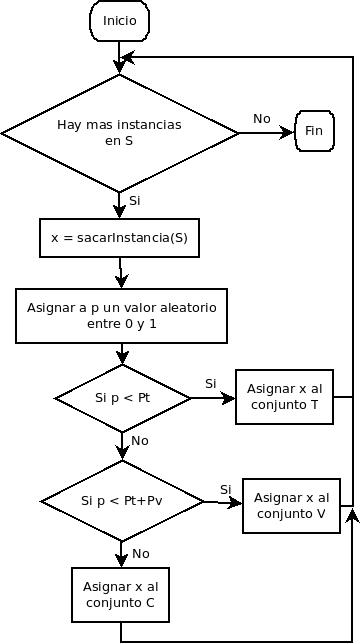
\includegraphics[width=7cm]{diagrams/setPartition.jpg}
\end{center}
\caption{Procedimiento para producir un conjunto de entrenamiento y validación}
\label{fig:setPartition}
\end{figure}

\subsection{Mediciones}
Una vez entrenado el modelo de distribución normal multivariable como se explicó en el capitulo \ref{chap:ml}, se procede a hacer las mediciones de precisión sobre datos no vistos en el proceso de entrenamiento. Para esto se usa el modelo entrenado y se observan las predicciones realizadas por este modelo sobre el conjunto de validación. Cabe recordar que el conjunto de validación esta etiquetado, y por esta razón, se conoce cual es la salida esperada para el dato con el que se esta probando el modelo. En terminos formales, el conjunto de entrenamiento $V$ se podría definir de la siguiente forma:
\[ V = \{\vec{x_i},r_i\}_{i=0}^N \]
Donde $N$ es la cantidad de elementos del conjunto de validación y $r_i$ es la salida esperada para el valor de entrada $\vec{x}_i$. Supongamos que la salida observada del modelo entrenado para el valor $\vec{x_i}$ es $y_i$. Entonces se considera que el clasificador comete un error si $r_i \ne y_i$ y acierta si $r_i = y_i$. Considerando que una igualdad tenga por valor 1 si es verdadera y 0 si es falsa, entonces el valor medido se calcula de la siguiente forma:
\[ A = \frac{ \sum_{j=0}^{N}(r_i=y_i) }{N} \]
Se puede observar que el valor medido $A$ significa la cantidad de aciertos sobre el número total de intentos de predicción. Y por tanto mide el porcentaje de efectividad del clasificador para el problema de reconocimiento de caracteres.

\chapter{Conclusiones y resultados}

\section{Primeros resultados}

\section{Mejoras realizadas}

\section{Resultados finales}

\section{Proyectos que se pueden derivar de esta investigación}

\chapter{GNU Free Documentation License}

0. PREÁMBULO

El propósito de esta Licencia es permitir que un manual, libro de texto, u otro documento escrito sea libre en el sentido de libertad: asegurar a todo el mundo la libertad efectiva de copiarlo y redistribuirlo, con o sin modificaciones, de manera comercial o no. En segundo término, esta Licencia proporciona al autor y al editor[2] una manera de obtener reconocimiento por su trabajo, sin que se le considere responsable de las modificaciones realizadas por otros.

Esta Licencia es de tipo copyleft, lo que significa que los trabajos derivados del documento deben a su vez ser libres en el mismo sentido. Complementa la Licencia Pública General de GNU, que es una licencia tipo copyleft diseñada para el software libre.

Hemos diseñado esta Licencia para usarla en manuales de software libre, ya que el software libre necesita documentación libre: un programa libre debe venir con manuales que ofrezcan la mismas libertades que el software. Pero esta licencia no se limita a manuales de software; puede usarse para cualquier texto, sin tener en cuenta su temática o si se publica como libro impreso o no. Recomendamos esta licencia principalmente para trabajos cuyo fin sea instructivo o de referencia.

1. APLICABILIDAD Y DEFINICIONES

Esta Licencia se aplica a cualquier manual u otro trabajo, en cualquier soporte, que contenga una nota del propietario de los derechos de autor que indique que puede ser distribuido bajo los términos de esta Licencia. Tal nota garantiza en cualquier lugar del mundo, sin pago de derechos y sin límite de tiempo, el uso de dicho trabajo según las condiciones aquí estipuladas. En adelante la palabra Documento se referirá a cualquiera de dichos manuales o trabajos. Cualquier persona es un licenciatario y será referido como Usted. Usted acepta la licencia si copia, modifica o distribuye el trabajo de cualquier modo que requiera permiso según la ley de propiedad intelectual.

Una Versión Modificada del Documento significa cualquier trabajo que contenga el Documento o una porción del mismo, ya sea una copia literal o con modificaciones y/o traducciones a otro idioma.

Una Sección Secundaria es un apéndice con título o una sección preliminar del Documento que trata exclusivamente de la relación entre los autores o editores y el tema general del Documento (o temas relacionados) pero que no contiene nada que entre directamente en dicho tema general (por ejemplo, si el Documento es en parte un texto de matemáticas, una Sección Secundaria puede no explicar nada de matemáticas). La relación puede ser una conexión histórica con el tema o temas relacionados, o una opinión legal, comercial, filosófica, ética o política acerca de ellos.

Las Secciones Invariantes son ciertas Secciones Secundarias cuyos títulos son designados como Secciones Invariantes en la nota que indica que el documento es liberado bajo esta Licencia. Si una sección no entra en la definición de Secundaria, no puede designarse como Invariante. El documento puede no tener Secciones Invariantes. Si el Documento no identifica las Secciones Invariantes, es que no las tiene.

Los Textos de Cubierta son ciertos pasajes cortos de texto que se listan como Textos de Cubierta Delantera o Textos de Cubierta Trasera en la nota que indica que el documento es liberado bajo esta Licencia. Un Texto de Cubierta Delantera puede tener como mucho 5 palabras, y uno de Cubierta Trasera puede tener hasta 25 palabras.

Una copia Transparente del Documento, significa una copia para lectura en máquina, representada en un formato cuya especificación está disponible al público en general, apto para que los contenidos puedan ser vistos y editados directamente con editores de texto genéricos o (para imágenes compuestas por puntos) con programas genéricos de manipulación de imágenes o (para dibujos) con algún editor de dibujos ampliamente disponible, y que sea adecuado como entrada para formateadores de texto o para su traducción automática a formatos adecuados para formateadores de texto. Una copia hecha en un formato definido como Transparente, pero cuyo marcaje o ausencia de él haya sido diseñado para impedir o dificultar modificaciones posteriores por parte de los lectores no es Transparente. Un formato de imagen no es Transparente si se usa para una cantidad de texto sustancial. Una copia que no es Transparente se denomina Opaca.

Como ejemplos de formatos adecuados para copias Transparentes están ASCII puro sin marcaje, formato de entrada de Texinfo, formato de entrada de LaTeX, SGML o XML usando una DTD disponible públicamente, y HTML, PostScript o PDF simples, que sigan los estándares y diseñados para que los modifiquen personas. Ejemplos de formatos de imagen transparentes son PNG, XCF y JPG. Los formatos Opacos incluyen formatos propietarios que pueden ser leídos y editados únicamente en procesadores de palabras propietarios, SGML o XML para los cuáles las DTD y/o herramientas de procesamiento no estén ampliamente disponibles, y HTML, PostScript o PDF generados por algunos procesadores de palabras sólo como salida.

La Portada significa, en un libro impreso, la página de título, más las páginas siguientes que sean necesarias para mantener, de manera legible, el material que esta Licencia requiere en la portada. Para trabajos en formatos que no tienen página de portada como tal, Portada significa el texto cercano a la aparición más prominente del título del trabajo, precediendo el comienzo del cuerpo del texto.

El Editor se refiere a cualquier persona o entidad que distribuya copias del Documento a el público.

Una sección Titulada XYZ significa una parte del Documento cuyo título es precisamente XYZ o contiene XYZ entre paréntesis, a continuación de texto que traduce XYZ a otro idioma (aquí XYZ se refiere a nombres de sección específicos mencionados más abajo, como Agradecimientos, Dedicatorias , Aprobaciones o Historia). Conservar el Título de tal sección cuando se modifica el Documento significa que permanece una sección Titulada XYZ según esta definición.[3]

El Documento puede incluir Limitaciones de Garantía cercanas a la nota donde se declara que al Documento se le aplica esta Licencia. Se considera que estas Limitaciones de Garantía están incluidas, por referencia, en la Licencia, pero sólo en cuanto a limitaciones de garantía: cualquier otra implicación que estas Limitaciones de Garantía puedan tener es nula y no tiene efecto en el significado de esta Licencia.

2. COPIA LITERAL

Usted puede copiar y distribuir el Documento en cualquier soporte, sea en forma comercial o no, siempre y cuando esta Licencia, las notas de copyright y la nota que indica que esta Licencia se aplica al Documento se reproduzcan en todas las copias y que usted no añada ninguna otra condición a las expuestas en esta Licencia. Usted no puede usar medidas técnicas para obstruir o controlar la lectura o copia posterior de las copias que usted haga o distribuya. Sin embargo, usted puede aceptar compensación a cambio de las copias. Si distribuye un número suficientemente grande de copias también deberá seguir las condiciones de la sección 3.

Usted también puede prestar copias, bajo las mismas condiciones establecidas anteriormente, y puede exhibir copias públicamente.

3. COPIADO EN CANTIDAD

Si publica copias impresas del Documento (o copias en soportes que tengan normalmente cubiertas impresas) que sobrepasen las 100, y la nota de licencia del Documento exige Textos de Cubierta, debe incluir las copias con cubiertas que lleven en forma clara y legible todos esos Textos de Cubierta: Textos de Cubierta Delantera en la cubierta delantera y Textos de Cubierta Trasera en la cubierta trasera. Ambas cubiertas deben identificarlo a Usted clara y legiblemente como editor de tales copias. La cubierta debe mostrar el título completo con todas las palabras igualmente prominentes y visibles. Además puede añadir otro material en las cubiertas. Las copias con cambios limitados a las cubiertas, siempre que conserven el título del Documento y satisfagan estas condiciones, pueden considerarse como copias literales.

Si los textos requeridos para la cubierta son muy voluminosos para que ajusten legiblemente, debe colocar los primeros (tantos como sea razonable colocar) en la verdadera cubierta y situar el resto en páginas adyacentes.

Si Usted publica o distribuye copias Opacas del Documento cuya cantidad exceda las 100, debe incluir una copia Transparente, que pueda ser leída por una máquina, con cada copia Opaca, o bien mostrar, en cada copia Opaca, una dirección de red donde cualquier usuario de la misma tenga acceso por medio de protocolos públicos y estandarizados a una copia Transparente del Documento completa, sin material adicional. Si usted hace uso de la última opción, deberá tomar las medidas necesarias, cuando comience la distribución de las copias Opacas en cantidad, para asegurar que esta copia Transparente permanecerá accesible en el sitio establecido por lo menos un año después de la última vez que distribuya una copia Opaca de esa edición al público (directamente o a través de sus agentes o distribuidores).

Se solicita, aunque no es requisito, que se ponga en contacto con los autores del Documento antes de redistribuir gran número de copias, para darles la oportunidad de que le proporcionen una versión actualizada del Documento.

4. MODIFICACIONES

Puede copiar y distribuir una Versión Modificada del Documento bajo las condiciones de las secciones 2 y 3 anteriores, siempre que usted libere la Versión Modificada bajo esta misma Licencia, con la Versión Modificada haciendo el rol del Documento, por lo tanto dando licencia de distribución y modificación de la Versión Modificada a quienquiera posea una copia de la misma. Además, debe hacer lo siguiente en la Versión Modificada:

A. Usar en la Portada (y en las cubiertas, si hay alguna) un título distinto al del Documento y de sus versiones anteriores (que deberían, si hay alguna, estar listadas en la sección de Historia del Documento). Puede usar el mismo título de versiones anteriores al original siempre y cuando quien las publicó originalmente otorgue permiso.
B. Listar en la Portada, como autores, una o más personas o entidades responsables de la autoría de las modificaciones de la Versión Modificada, junto con por lo menos cinco de los autores principales del Documento (todos sus autores principales, si hay menos de cinco), a menos que le eximan de tal requisito.
C. Mostrar en la Portada como editor el nombre del editor de la Versión Modificada.
D. Conservar todas las notas de copyright del Documento.
E. Añadir una nota de copyright apropiada a sus modificaciones, adyacente a las otras notas de copyright.
F. Incluir, inmediatamente después de las notas de copyright, una nota de licencia dando el permiso para usar la Versión Modificada bajo los términos de esta Licencia, como se muestra en el Apéndice [Apéndice] al final de este documento.
G. Conservar en esa nota de licencia el listado completo de las Secciones Invariantes y de los Textos de Cubierta que sean requeridos en la nota de Licencia del Documento original.
H. Incluir una copia sin modificación de esta Licencia.
I. Conservar la sección Titulada Historia, conservar su Título y añadirle un elemento que declare al menos el título, el año, los nuevos autores y el editor de la Versión Modificada, tal como figuran en la Portada. Si no hay una sección Titulada Historia en el Documento, crear una estableciendo el título, el año, los autores y el editor del Documento, tal como figuran en su Portada, añadiendo además un elemento describiendo la Versión Modificada, como se estableció en la oración anterior.
J. Conservar la dirección en red, si la hay, dada en el Documento para el acceso público a una copia Transparente del mismo, así como las otras direcciones de red dadas en el Documento para versiones anteriores en las que estuviese basado. Pueden ubicarse en la sección Historia. Se puede omitir la ubicación en red de un trabajo que haya sido publicado por lo menos cuatro años antes que el Documento mismo, o si el editor original de dicha versión da permiso.
K. En cualquier sección Titulada Agradecimientos o Dedicatorias, conservar el Título de la sección y conservar en ella toda la sustancia y el tono de los agradecimientos y/o dedicatorias incluidas por cada contribuyente.
L. Conservar todas las Secciones Invariantes del Documento, sin alterar su texto ni sus títulos. Números de sección o el equivalente no son considerados parte de los títulos de la sección.
M. Borrar cualquier sección titulada Aprobaciones. Tales secciones no pueden estar incluidas en las Versiones Modificadas.
N. No cambiar el título de ninguna sección existente a Aprobaciones ni a uno que entre en conflicto con el de alguna Sección Invariante.
O. Conservar todas las Limitaciones de Garantía.
Si la Versión Modificada incluye secciones o apéndices nuevos que califiquen como Secciones Secundarias y contienen material no copiado del Documento, puede opcionalmente designar algunas o todas esas secciones como invariantes. Para hacerlo, añada sus títulos a la lista de Secciones Invariantes en la nota de licencia de la Versión Modificada. Tales títulos deben ser distintos de cualquier otro título de sección.

Puede añadir una sección titulada Aprobaciones, siempre que contenga únicamente aprobaciones de su Versión Modificada por otras fuentes --por ejemplo, observaciones de peritos o que el texto ha sido aprobado por una organización como la definición oficial de un estándar.

Puede añadir un pasaje de hasta cinco palabras como Texto de Cubierta Delantera y un pasaje de hasta 25 palabras como Texto de Cubierta Trasera en la Versión Modificada. Una entidad solo puede añadir (o hacer que se añada) un pasaje al Texto de Cubierta Delantera y uno al de Cubierta Trasera. Si el Documento ya incluye un textos de cubiertas añadidos previamente por usted o por la misma entidad que usted representa, usted no puede añadir otro; pero puede reemplazar el anterior, con permiso explícito del editor que agregó el texto anterior.

Con esta Licencia ni los autores ni los editores del Documento dan permiso para usar sus nombres para publicidad ni para asegurar o implicar aprobación de cualquier Versión Modificada.

5. COMBINACIÓN DE DOCUMENTOS

Usted puede combinar el Documento con otros documentos liberados bajo esta Licencia, bajo los términos definidos en la sección 4 anterior para versiones modificadas, siempre que incluya en la combinación todas las Secciones Invariantes de todos los documentos originales, sin modificar, listadas todas como Secciones Invariantes del trabajo combinado en su nota de licencia. Así mismo debe incluir la Limitación de Garantía.

El trabajo combinado necesita contener solamente una copia de esta Licencia, y puede reemplazar varias Secciones Invariantes idénticas por una sola copia. Si hay varias Secciones Invariantes con el mismo nombre pero con contenidos diferentes, haga el título de cada una de estas secciones único añadiéndole al final del mismo, entre paréntesis, el nombre del autor o editor original de esa sección, si es conocido, o si no, un número único. Haga el mismo ajuste a los títulos de sección en la lista de Secciones Invariantes de la nota de licencia del trabajo combinado.

En la combinación, debe combinar cualquier sección Titulada Historia de los documentos originales, formando una sección Titulada Historia; de la misma forma combine cualquier sección Titulada Agradecimientos, y cualquier sección Titulada Dedicatorias. Debe borrar todas las secciones tituladas Aprobaciones.

6. COLECCIONES DE DOCUMENTOS

Puede hacer una colección que conste del Documento y de otros documentos liberados bajo esta Licencia, y reemplazar las copias individuales de esta Licencia en todos los documentos por una sola copia que esté incluida en la colección, siempre que siga las reglas de esta Licencia para cada copia literal de cada uno de los documentos en cualquiera de los demás aspectos.

Puede extraer un solo documento de una de tales colecciones y distribuirlo individualmente bajo esta Licencia, siempre que inserte una copia de esta Licencia en el documento extraído, y siga esta Licencia en todos los demás aspectos relativos a la copia literal de dicho documento.

7. AGREGACIÓN CON TRABAJOS INDEPENDIENTES

Una recopilación que conste del Documento o sus derivados y de otros documentos o trabajos separados e independientes, en cualquier soporte de almacenamiento o distribución, se denomina un agregado si el copyright resultante de la compilación no se usa para limitar los derechos de los usuarios de la misma más allá de lo que los de los trabajos individuales permiten. Cuando el Documento se incluye en un agregado, esta Licencia no se aplica a otros trabajos del agregado que no sean en sí mismos derivados del Documento.

Si el requisito de la sección 3 sobre el Texto de Cubierta es aplicable a estas copias del Documento y el Documento es menor que la mitad del agregado entero, los Textos de Cubierta del Documento pueden colocarse en cubiertas que enmarquen solamente el Documento dentro del agregado, o el equivalente electrónico de las cubiertas si el documento está en forma electrónica. En caso contrario deben aparecer en cubiertas impresas enmarcando todo el agregado.

8. TRADUCCIÓN

La Traducción es considerada como un tipo de modificación, por lo que usted puede distribuir traducciones del Documento bajo los términos de la sección 4. El reemplazo las Secciones Invariantes con traducciones requiere permiso especial de los dueños de derecho de autor, pero usted puede añadir traducciones de algunas o todas las Secciones Invariantes a las versiones originales de las mismas. Puede incluir una traducción de esta Licencia, de todas las notas de licencia del documento, así como de las Limitaciones de Garantía, siempre que incluya también la versión en Inglés de esta Licencia y las versiones originales de las notas de licencia y Limitaciones de Garantía. En caso de desacuerdo entre la traducción y la versión original en Inglés de esta Licencia, la nota de licencia o la limitación de garantía, la versión original en Inglés prevalecerá.

Si una sección del Documento está Titulada Agradecimientos, Dedicatorias o Historia el requisito (sección 4) de Conservar su Título (Sección 1) requerirá, típicamente, cambiar su título.

9. TERMINACIÓN

Usted no puede copiar, modificar, sublicenciar o distribuir el Documento salvo por lo permitido expresamente bajo esta Licencia. Cualquier intento en otra manera de copia, modificación, sublicenciamiento, o distribución de él es nulo, y dará por terminados automáticamente sus derechos bajo esa Licencia.

Sin embargo, si usted cesa toda violación a esta Licencia, entonces su licencia proveniente de un titular de copyright queda restaurada (a) provisionalmente, a menos y hasta que el titular del copyright explícita y finalmente termine su licencia, y (b) permanentemente, si el titular del copyright falla en notificarle de la violación por algún medio razonable en un tiempo menor a 60 días después del cese.

Además, su licencia proveniente de un titular del copyright particular queda restaurada permanentemente si el titular del copyright le notifica de la violación por algún método razonable, es la primera vez que usted ha recibido aviso de la violación de esta Licencia (para cualquier trabajo) de ese titular del copyright, y usted remedia la violación en un tiempo menor a 30 días después de recibir dicho aviso.

La terminación de sus derechos bajo ésta sección no termina la licencia de terceros que hayan recibido copias o derechos de usted bajo ésta Licencia. Si sus derechos han sido terminados y no restaurados permanentemente, recibir una copia de alguna parte o el total del mismo material no le da ningún derecho de usarlo.

10. REVISIONES FUTURAS DE ESTA LICENCIA

De vez en cuando la Free Software Foundation puede publicar versiones nuevas y revisadas de la Licencia de Documentación Libre GNU. Tales versiones nuevas serán similares en espíritu a la presente versión, pero pueden diferir en detalles para solucionar nuevos problemas o intereses. Vea http://www.gnu.org/copyleft/.

Cada versión de la Licencia tiene un número de versión que la distingue. Si el Documento especifica que se aplica una versión numerada en particular de esta licencia o cualquier versión posterior, usted tiene la opción de seguir los términos y condiciones de la versión especificada o cualquiera posterior que haya sido publicada (no como borrador) por la Free Software Foundation. Si el Documento no especifica un número de versión de esta Licencia, puede escoger cualquier versión que haya sido publicada (no como borrador) por la Free Software Foundation. Si el Documento especifica que un apoderado puede decidir qué versión futura de esta Licencia puede ser utilizada, esa frase de aceptación del apoderado de una versión le autoriza permanentemente a escoger esa versión para el Documento.

11. Re-Licenciamiento

Un Sitio de Colaboración Masiva Multiautor (o Sitio CMM) significa cualquier servidor World Wide Web que publique trabajos que puedan ser sujetos a copyright y que también provea medios prominentes para que cualquiera pueda editar esos trabajos. Una Wiki pública que cualquiera puede editar es un ejemplo de tal servidor. Una Colaboración Masiva Multiautor (o CMM) contenida en el sitio significa cualquier colección de trabajos que puedan ser sujetos a copyright publicados en el sitio de CMM.

CC-BY-SA significa la licencia Creative Commons Attribution-Share Alike 3.0 (Reconocimiento-Compartir bajo la misma licencia 3.0 de Creative Commons) publicada por Creative Commons Corporation, una corporación sin fines de lucro con base en San Francisco, California, así como versiones futuras copyleft de esa licencia publicada por esa misma organización.

Incorporar significa publicar o re-publicar un Documento, como un todo o parcialmente, como parte de otro Documento.

Un sitio CMM es elegible para re-licenciamiento si es licenciado bajo esta Licencia, y si todos los trabajos que fueron publicados originalmente bajo esta Licencia en algún otro lugar diferente a esta CMM, y subsecuentemente incorporado como un todo o parcialmente a la CMM, (1)no tenía textos de cubierta o secciones invariantes, y (2) fueron incorporados previo a Noviembre 1, 2008.

El operador de un Sitio CMM puede volver a publicar una CMM contenida en el sitio bajo CC-BY-SA en el mismo sitio en cualquier momento antes de Agosto 1, 2009, siempre que la CMM sea elegible para re-licenciamiento.

\chapter{Bibliografía}

Everitt, B.S. (2006) The Cambridge Dictionary of Statistics, Third Edition. pp. 313–314. Cambridge University Press, Cambridge. ISBN 0521690277

Weisstein, Eric W. "Probability Density Function." From MathWorld--A Wolfram Web Resource. http://mathworld.wolfram.com/ProbabilityDensityFunction.html

\end{document}
